\ifx\mainclass\undefined
\documentclass[cn,11pt,chinese,black,simple]{elegantbook}
\usepackage{pdfpages}
% 微分号
\newcommand{\dd}[1]{\mathrm{d}#1}
\newcommand{\pp}[1]{\partial{}#1}

% FT LT ZT
\newcommand{\dtft}[1]{\text{DTFT}[#1]}
\newcommand{\dtftr}[1]{\text{DTFT}^{-1}[#1]}
\newcommand{\dtfta}{\xrightarrow{\text{DTFT}}}

\newcommand{\where}[1]{\Big|_{#1}}
\newcommand{\abs}[1]{\left| #1 \right|}
\newcommand{\zt}[1]{\mathscr{Z}[#1]}
\newcommand{\ztr}[1]{\mathscr{Z}^{-1}[#1]}
\newcommand{\zta}{\xrightarrow{\mathscr{Z}}} 
\newcommand{\lt}[1]{\mathscr{L}[#1]}
\newcommand{\lta}{\xrightarrow{\mathscr{L}}} 
\newcommand{\ft}[1]{\mathscr{F}[#1]}
\newcommand{\fta}{\xrightarrow{\mathscr{F}}} 
\newcommand{\dsum}{\displaystyle\sum}
\newcommand{\aint}{\int_{-\infty}^{+\infty} }

% 积分求和号

% 简易图片插入
\newcommand{\qfig}[3][nolabel]{
  \begin{figure}[!htb]
      \centering
      \includegraphics[width=0.6\textwidth]{#2}
      \caption{#3}
      \label{#1}
  \end{figure}
}

\usepackage{pdfpages}
\includepdfset{pagecommand=\thispagestyle{plain}}
% 表格
\renewcommand\arraystretch{1.5}

\usepackage{shapepar}
\usepackage{longtable}
% 日期

\begin{document}
\fi 
\def\chapname{review}



% Start Here

\chapter{离散信号与系统}

\section{因果性、记忆性}

是否用到了 \(x[n]\) 的未来值/过去值,而不是其他可计算的值。

\section{LTI 系统}

既是线性系统,又是时不变系统,称为LTI系统。其\textbf{充要条件}是 \(y[n] = x[n] \otimes h[n]\) 。

无法直接判断可以假设是一个 LTI 系统: 

\[\frac{1}{2^n} \rightarrow \frac{1}{4^n}\] 

假设是:

 \begin{itemize}
     \item LTI:\[y[n] = \asum h[k] \frac{1}{2^{n-k}} = \frac{1}{2^n} h_1[k]\] 矛盾!
     \item TI and Linear: \[\begin{aligned}
        \frac{1}{2^{n-1}} &\rightarrow \frac{1}{4^{n-1}} \\
        2 \frac{1}{2^n} &\rightarrow 4 \frac{1}{4^n}
     \end{aligned}\]
 \end{itemize}

\subsection{因果系统}

\(h[n] = h[n] u[n]\) 

\subsection{稳定系统}

\[
\dsum_{-\infty}^{+\infty} |h(n)| =M<+\infty
\]

\subsection{特征频率与 LTI 系统}

若是有一个无限长的指数信号,那么有一个单频信号:

2.27

\[
    \left[e^{j \omega_{0} n}\right]\rightarrow \dsum_{k=-\infty}^{+\infty} 2 \pi \delta\left(\omega-\omega_{0}+2 k \pi\right)
\]

但是若是有限长,那么就有引入除去 \(\omega_0\) 的分量,因此对于一个 LTI 系统来说,放大 \(e^{j \omega_0 n}\) 和 \(e^{j \omega_0 n} u[n]\) 需要的系统函数是不一样的。

\section{差分方程的阶数}

输出 \(y[n-i]\) 最高值和最低值 \(i\) 的差值。

LCCDE = linear constant-coefficient difference equation .



\chapter{DTFT 变换}


\section{频域阶数}

2.42

若是在原有的系统函数多一个 \(z\) ,说明原来 \(a_0 z^0\) 的位置变成了 \(a_0 z^1\) ,也就是 \(a_n\) 变成了 \(a_{n+1}\) 。 同理 \(z^{-1}\) 对应 \(a_{n-1}\) 。由于使用因果信号, \(z^{-1}\) 的形式更合适。

\section{系统设计}

2.56 ,

需要一个系统时,可以通过其定义入手,配凑式子。 同时,对于特定的频率分量,其幅度、角度变换是由其频率响应改变的。

\section{DTFT 推导细节}

\[
\begin{aligned}
D T F T^{-1}\left[X\left(e^{j \omega}\right)\right]&=\dfrac{1}{2 \pi} \int_{-\pi}^{\pi} X\left(e^{j \omega}\right) e^{j \omega n} d \omega \\
&=\dfrac{1}{2 \pi} \int_{-\pi}^{\pi}\left(\dsum_{k=-\infty}^{+\infty} x(k) e^{-j \omega k}\right) e^{j \omega n} d \omega \\
&=\dsum_{k=-\infty}^{+\infty} x(k) \dfrac{1}{2 \pi} \int_{-\pi}^{\pi} e^{-j \omega(k-n)} d \omega\\
&=\dsum_{k=-\infty}^{+\infty} x(k) \delta(k-n)=x(n)
\end{aligned}
\]

注意  \(2\pi\) 与 \(\delta(n)\) 的由来:单位虚数的积分。

将 IDTFT 展开成累加的形式,实际上是将不同频率的分量逐个恢复:

\begin{align*}
    \begin{array}{l}
    X(n)=\dfrac{1}{2 \pi} \int_{-\pi}^{\pi} X\left(e^{j \omega}\right) e^{j \omega n} d \omega \\
    =\dfrac{1}{2 \pi} \dsum_{-\infty}^{+\infty} X\left(e^{j k \Delta \omega}\right) e^{j k \Delta \omega n} \Delta \omega=\dsum_{-\infty}^{+\infty} \dfrac{\left[X\left(e^{j k \Delta \omega}\right) \Delta \omega\right]}{2 \pi} e^{j k \Delta \omega n}
    \end{array}
\end{align*}



\begin{longtable}{ll} 
    \caption{DTFT 变换对} \\ 
    \toprule
    时域函数 & DTFT  \\
    \midrule
    \endfirsthead
    
    \toprule
    时域函数 & DTFT  \\
    \midrule
    \endhead 
  
    \hline
    \multicolumn{2}{c}{见下页}\\   \bottomrule
    \endfoot
  
    \bottomrule
    \endlastfoot
    \(\delta(n)\) & 1\\
    \(1\) & \(\dsum_{k=-\infty}^{+\infty} 2 \pi \delta(\omega+2 k \pi)\) \\ 
    \(u(n)\) & \(\dfrac{1}{1-e^{-j \omega}}+\dsum_{k=-\infty}^{+\infty} \pi \delta(\omega+2 k \pi)\)  \\
    \(e^{j\omega_0 n}\) & \(
        \dsum_{k=-\infty}^{+\infty} 2 \pi \delta\left(\omega-\omega_{0}+2 k \pi\right)
        \)\\
    \(W_N(n)\) & \(\dfrac{\sin \left(\dfrac{\omega N}{2}\right)}{\sin \left(\dfrac{\omega}{2}\right)} e^{-j \dfrac{(N-1) \omega}{2}}\) \\
    \(\dfrac{w_{c}}{\pi} \dfrac{\sin \left[w_{c}(n-\alpha)\right]}{w_{c}(n-\alpha)}\)  & \(e^{-j\omega\alpha} (u(\omega+\omega_c) - u(\omega-\omega_c))\)\\ 
\end{longtable}


\begin{longtable}{ll} 
    \caption{DTFT 变换性质} \\ 
    \toprule
    性质名称 & 表达式  \\
    \midrule
    \endfirsthead
    
    \toprule
    性质名称 & 表达式  \\
    \midrule
    \endhead 
  
    \hline
    \multicolumn{2}{c}{见下页}\\   \bottomrule
    \endfoot
  
    \bottomrule
    \endlastfoot
    线性 & \\ 
    时域平移-频域调制 &  \(x(n-m) \rightarrow e^{-j w m} X\left(e^{j w}\right)\) \\
    时域调制-频域平移 & \(e^{j n w} x(n) \quad \rightarrow  X\left(e^{j\left(w-w_{0}\right)}\right)\) \\ 
    时域翻折 & \(x(-n) \rightarrow X(e^{-j \omega})\) \\ 
    帕塞瓦尔定理 & \(\begin{aligned}
        \dsum_{n=-\infty}^{\infty} x(n) y^{*}(n) &=\dfrac{1}{2 \pi} \int_{-\pi}^{\pi} X\left(e^{j w}\right) Y^{*}\left(e^{j w}\right) d w \\
        \dsum_{n=-\infty}^{\infty}|x(n)|^{2}&=\dfrac{1}{2 \pi} \int_{-\pi}^{\pi}\left|X\left(e^{j w}\right)\right|^{2} d w
        \end{aligned}\) \\
\end{longtable}

可以利用帕赛瓦尔定理解决一些求和式子:Slide P83.



\section{DTFT 对称性}

共轭对称与共轭反对称序列定义,实际上是实部、虚部分别的奇偶对称: \[
    \begin{array}{l}
    x_{e}(n)=x_{e}^{*}(-n) \\
    x_{o}(n)=-x_{o}^{*}(-n)
    \end{array}
\]

任意序列都可以进行共轭分解:

\[\begin{aligned}
    x(n) &= x_e(n) + x_o(n) \\ 
    x(-n) &= x_e(-n) + x_o(-n) = x_e^*(n) - x_o^*(n) 
\end{aligned}\]

\[
\begin{array}{l}
x_{e}(n)=\dfrac{1}{2}\left[x(n)+x^{*}(-n)\right] \\
x_{o}(n)=\dfrac{1}{2}\left[x(n)-x^{*}(-n)\right]
\end{array}
\]

根据下一小节的性质:

\[
\begin{array}{l}
X_{e}\left(e^{j \omega}\right)=\dfrac{1}{2}\left[X\left(e^{j \omega}\right)+X^{*}\left(e^{-j \omega}\right)\right] \\
X_{o}\left(e^{j \omega}\right)=\dfrac{1}{2}\left[X\left(e^{j \omega}\right)-X^{*}\left(e^{-j \omega}\right)\right]
\end{array}
\]

同样的对频域函数进行变换:

\[X(e^{j\omega}) = X_e(e^{j\omega}) + X_o(e^{-j\omega})\] 

\[
\begin{array}{l}
X_{e}\left(e^{j \omega}\right)=\dfrac{1}{2}\left[X\left(e^{j \omega}\right)+X^{*}\left(e^{-j \omega}\right)\right] \\
X_{o}\left(e^{j \omega}\right)=\dfrac{1}{2}\left[X\left(e^{j \omega}\right)-X^{*}\left(e^{-j \omega}\right)\right]
\end{array}
\]

逆变换:
\[
\begin{array}{l}
D T F T\{\operatorname{Re}[x(n)]\}=X_{e}\left(e^{j \omega}\right) \\
D T F T\{j \operatorname{Im}[x(n)]\}=X_{o}\left(e^{j \omega}\right)
\end{array}
\]
\section{变换共轭性质}

具有普适性。

\[
\begin{array}{c}
\mathcal{Z}\left[x^{*}[n]\right]=\dsum_{n=-\infty}^{\infty} x^{*}[n] z^{-n}=\left(\dsum_{n=-\infty}^{\infty} x[n]\left(z^{*}\right)^{-n}\right)^{*}=X^{*}\left(z^{*}\right) \\
\mathcal{Z}[x[-n]]=\dsum_{n=-\infty}^{\infty} x[-n] z^{-n}=\dsum_{n=-\infty}^{\infty} x[n]\left(z^{-1}\right)^{-n}=X\left(z^{-1}\right) \\
\mathcal{Z}[\operatorname{Re}\{x[n]\}]=\mathcal{Z}\left[\dfrac{x[n]+x^{*}[n]}{2}\right]=\dfrac{1}{2}\left[X(z)+X^{*}\left(z^{*}\right)\right] \\
\mathcal{Z}[\operatorname{Im}\{x[n]\}]=\mathcal{Z}\left[\dfrac{z[n]-x^{*}[n]}{2 j}\right]=\dfrac{1}{2 j}\left[X(z)-X^{*}\left(z^{*}\right)\right]
\end{array}
\]

\section{Z 变换}


\begin{longtable}{lll} 
    \caption{\(\mathscr{Z}\)变换对} \\ 
    \toprule
    时域函数 & \(z\)域函数 & ROC \\
    \midrule
    \endfirsthead
    
    \toprule
    时域函数 & \(z\)域函数 & ROC \\
    \midrule
    \endhead 
  
    \hline
    \multicolumn{3}{c}{见下页}\\   \bottomrule
    \endfoot
  
    \bottomrule
    \endlastfoot
    \(\delta(n)\) & 1 & 全平面\\
    \(u(n)\) & \(\dfrac{z}{z-1}\) & \(\abs{z}>1\) \\
    \(a^n u(n)\) & \(\dfrac{z}{z-a}\) & \(\abs{z}>a\) \\
    \(-a^n u(-n-1)\) & \(\dfrac{z}{z-a}\) & \(\abs{z}<a\)\\
    \(\cos(\omega_0 n)u(n)\) & \(\dfrac{z^2-z \cos \omega_0}{z^2 - 2 z \cos\omega_0 + 1}\) & \(\abs{z}>1\) \\
    \(\sin(\omega_0 n)u(n)\) & \(\dfrac{z \sin\omega_0}{z^2 -2 z \cos\omega_0 + 1}\) &  \(\abs{z}>1\) \\

\end{longtable}
  


\begin{longtable}{llll} 
    \caption{\(\mathscr{Z}\)变换性质} \\ 
    \toprule
    时域函数 & \(z\)域函数 & 原ROC  & 变换后ROC\\
    \midrule
    \endfirsthead
    
    \toprule
    时域函数 & \(z\)域函数 & 原ROC  & 变换后ROC\\
    \midrule
    \endhead 
  
    \hline
    \multicolumn{4}{c}{见下页}\\   \bottomrule
    \endfoot
  
    \bottomrule
    \endlastfoot
    \(x(-n)\) & \(X(z^{-1})\) & \(\alpha < \abs{z} < \beta\) & \(\dfrac{1}{\beta} < \abs{z} < \dfrac{1}{\alpha}\)\\
    \(x(\dfrac{n}{a}),a>0\) & \(X(z^a)\) & \(\alpha < \abs{z} < \beta\) & \(\alpha^{1/a} < \abs{z} < \beta^{1/a}\) \\
    \(x(n \pm m)\) & 双边 \(z^{\pm m}X(z)\) &  \(\alpha < \abs{z} < \beta\) &  \(\alpha < \abs{z} < \beta\) \\
    \(x(n - m)u(n)\) & 单边 \(z^{-m} \left[X(z) + \dsum_{k=-m}^{-1}x(k)z^{-k}\right]\) & \(\abs{z} > a\) & \(\abs{z} > a\) \\
    \(x(n + m)u(n)\) & 单边 \(z^{m} \left[X(z) - \dsum_{k=0}^{m-1}x(k)z^{-k}\right]\) & \(\abs{z} > a\) & \(\abs{z} > a\) \\
    线性性 & & & 原收敛域的交集 \\
    \(n x(n)\) & \(-z \dfrac{\dd{X(z)}}{\dd{z}}\) & \(\alpha < \abs{z} < \beta\) & \(\alpha < \abs{z} < \beta\)\\
    \(n^m x(n)\) & \(\left[-z\dfrac{\dd{}}{\dd{z}}\right]^m X(z)\) & \(\alpha < \abs{z} < \beta\) & \(\alpha < \abs{z} < \beta\)\\
    \(a^n x(n)\) & \(X(\dfrac{z}{a})\) &  \(\alpha < \abs{z} < \beta\) &  \(\alpha < \abs{\dfrac{z}{a}} < \beta\) \\
    \(x_1(n) \otimes x_2(n)\) & \(X_1(z) X_2(z)\) & & 原收敛域交集 \\
    \(x_1(n)x_2(n)\) & \(\dfrac{1}{2 \pi j}\displaystyle\oint_C X_1(\dfrac{z}{v})X_2(v) v^{-1} \dd{v} \)\footnote{其中\(C\)是\(X_1(\dfrac{z}{v})X_2(v)\) 收敛域交集内的逆时针方向围线} & & 收敛域是边界的乘积 \\
\end{longtable}

初值定理 \[\lim _{z \rightarrow \infty} X(z)=\lim _{z \rightarrow \infty} \dsum_{n=0}^{\infty} x(n) z^{-n}=x(0)\]

终值定理 \[\lim_{z\rightarrow 1}(z-1)X(z) = x(\infty)\]

帕塞瓦尔定理

\[
\left.Y(z)\right|_{z=1}=\dsum_{n=-\infty}^{+\infty} x(n) h^{*}(n)=\dfrac{1}{2 \pi j} \oint_{c} X(v) H^{*}\left(\dfrac{1}{V^{*}}\right)_{V}^{-1} d V
\]

\section{逆 Z 变换}

\subsection{部分分式法}

对于有理多项式 \[
    X(z)=\dfrac{B(z)}{A(z)}=\dfrac{b_{m} z^{m}+b_{m-1} z^{m-1}+\cdots+b_{1} z+b_{0}}{a_{n} z^{n}+a_{n-1} z^{n-1}+\cdots+a_{1} z+a_{0}}
\]
对于分解得到的 \(\dfrac{k z}{z-a}\)

\[
\begin{aligned}
    &k a^n u(n), \abs{z} > a\\
    &-k a^n u(-n-1), \abs{z} < a\\
\end{aligned}    
\]

\section{从能量看 Z 变换与 DTFT} 

时域频域的能量是一致的,没有发生衰减。


\section{Z 变换与时域频域}

为了解决非零状态系统,使用单边 Z 变换。

系统不改变频率:

\[
\begin{array}{l}
y(n)=x(n)^{*} h(n) \\
=\dsum_{m=-\infty}^{+\infty} h(m) e^{j\left[\omega_{0}(n-m)+\phi\right]}=e^{j\left[\omega_{0} n+\phi\right]} \dsum_{m=-\infty}^{+\infty} h(m) e^{-j \omega_{0} m} \\
=e^{j\left[\omega_{0} n+\phi\right]} H\left(e^{j \omega_{0}}\right)=x(n) H\left(e^{j \omega_{0}}\right)
\end{array}
\]

\section{系统零极点与频率响应}

\textbf{单位圆}上的系统函数是频率响应。

\subsection{幅度响应}

\begin{itemize}
    \item 原点处的零极点幅度无影响
    \item 经过单位圆上的零点幅度归零,单位圆附近的零点出现谷点
    \item 经过单位圆上的极点幅度无穷大,单位圆附近的极点出现峰点
    \item 远离零极点时影响较小
\end{itemize}

\subsection{相位响应}

\begin{itemize}
    \item 原点处的零极点对相位影响为线性,极点会引起滞后,零点会引起超前
    \item 靠近单位圆的零极点会引起较大的波动
    \item 远离极点零点的位置变换比较平缓
    \item 单位圆外部零点或极点造成相位连续增长,而单位圆内零极点对相位影响则随频率周期性归零
\end{itemize}

对于圆内外零极点:

\begin{itemize}
    \item 圆内极点:顺时针经过,相位迅速延后
    \item 圆外极点:顺时针经过,相位迅速提前
    \item 圆内零点:顺时针经过:相位迅速提前
    \item 圆外零点:顺时针经过:相位迅速延后
\end{itemize}

过单位圆零点相位突变 \(\pi\) 。

\section{LTI 系统幅相特性分析}

当给定幅度特性时,总可以通过共轭分解找到一个系统满足要求:
 

\[
\left|H\left(e^{j \omega}\right)\right|^{2}=H\left(e^{j \omega}\right) H *\left(e^{j \omega}\right)=\left.H(z) H^{*}\left(\dfrac{1}{z^{*}}\right)\right|_{z=e^{j \omega}}
\]

\subsection{全通系统}

频响恒为 \(1\) ,其零极点分别为 \(a\) 与 \(1/a^*\): 

\[
H_{a p}(z)=\dfrac{z^{-1}-a^{*}}{1-a z^{-1}}=-a^{*}\left(\dfrac{z-\dfrac{1}{a^{*}}}{z-a}\right)
\]

其相位响应为:群延迟为正值,连续相位递减。


\[
\begin{aligned}
&\text { Assume: } \quad a=r e^{j \theta}\\
&\arg \left[H_{a p}\left(e^{j \omega}\right)\right]\\
&=-\omega-2 \operatorname{arctg}\left[\dfrac{r \sin (\omega-\theta)}{1-r \cos (\omega-\theta)}\right]\\
&g r d\left[H_{a p}\left(e^{j \omega}\right)\right]\\
&=\dfrac{1-r^{2}}{\left|1-r e^{-j(\omega-\theta)}\right|^{2}}
\end{aligned}
\]

用途:

\begin{itemize}
    \item 相位均衡器,用于提高群延迟
    \item 任何因果稳定系统均可以分解为全通系统和最小相位的级联
    \item 若是系统不稳定,可以用于交换系统的零极点,而不改变幅度特性
\end{itemize}


\subsection{最小相位系统}

要求极点在单位圆内(主要考虑系统稳定性),要求零点在单位圆内(主要考虑相位变化最小)。

最小相位系统零极点均在单位圆内,极点往往与系统稳定性联系在一起,零点则往往与系统的延时特性联系在一起。逆系统也是因果稳定的,可以实现幅度和相位失真的完全补偿。

\begin{itemize}
    \item 最小相位延迟,全通系统总是使最小相位系统的连续相位减小:\[
        \begin{aligned}
            H(z)&=H_{\min }(z) H_{a p}(z)\\ 
            \arg \left[H\left(e^{j \omega}\right)\right]&=\arg \left[H \min \left(e^{j \omega}\right)\right]+\arg \left[H_{a p}\left(e^{j \omega}\right)\right] \\
            \arg \left[H\left(e^{j \omega}\right)\right] &\leq \arg \left[H_{\min }\left(e^{j \omega}\right)\right] \\
            \left|\arg \left[H\left(e^{j \omega}\right)\right]\right| &\geq\left|\arg \left[H_{\min }\left(e^{j \omega}\right)\right]\right| 
        \end{aligned}
        \]
    \item 最小群延迟,全通系统的群延迟对于所有的频率皆为正值:\[
    \begin{aligned}
        \operatorname{grd}\left[H\left(e^{j \omega}\right)\right]&=\operatorname{grd}\left[H_{\min }\left(e^{j \omega}\right)\right]+\operatorname{grd}\left[H_{a p}\left(e^{j \omega}\right)\right]\\
        \operatorname{grd}\left[H\left(e^{j \omega}\right)\right] &\geq \operatorname{grd}\left[H_{\min }\left(e^{j \omega}\right)\right]
    \end{aligned}
        \]
    \item 最小能量延迟,最集中在 \(n = 0\) 范围内:\[
        \dsum_{m=0}^{n}|h(n)|^{2} \leq \dsum_{m=0}^{n}\left|h_{\min }(m)\right|^{2}
        \] 
        因此:\[
            |h(0)| \leq\left|h_{\min }(0)\right|
            \]
\end{itemize}

最大能量延迟则发生在全部零点位于单位圆外的系统,因此该系统也称为最大相位系统。

\subsection{系统的补偿}

幅度失真由最小相位因子补偿,相位失真利用全通因子补偿特定频段。

\subsection{线性相位系统}

定义:群延迟 \(\alpha\) 为常数 \(\phi(\omega) = - \alpha \omega + \beta\)

线性相位响应时域表现为信号平移,波形不发生失真。

不考虑幅度响应条件下,线性相位系统即是所要寻找的物理可实现的无失真传输系统。

若是群延迟 \(\alpha\) 满足 \(2 \alpha\) 为整数,那么单位冲激响应严格对称,否则不严格对称,但是仍满足线性相位。

\subsection{广义线性相位系统}



在系统相位存在突变以及固定相位时,仍然存在恒定群延迟。

已知线性相位系统存在对称性,进行分析:

\[
\begin{aligned}
H\left(e^{j \omega}\right) &=A(\omega) e^{-j(\omega \alpha-\beta)} \\
D T F T \quad[h(\alpha-n)]=H\left(e^{-j \omega}\right) e^{-j \omega \alpha} &=A(\omega) e^{j \beta} \\
D T F T \quad[h(n+\alpha)]=H\left(e^{j \omega}\right) e^{j \omega \alpha} &=A(-\omega) e^{j \beta}
\end{aligned}
\]

因此,\(A(\omega)\) 的对称性决定了 \(h(n)\) 的对称性(一致)。

根据对称形式与 \(2 \alpha\) 的奇偶性,有四类 FIR 线性相位滤波器。

对称冲激响应的系统特性推导:

\[
    \begin{aligned}
h(n)&=\pm h(N-1-n) \quad 0 \leq n \leq N-1 \\
H(z)&=\dsum_{n=0}^{N-1} h(n) z^{-n}=\dsum_{n=0}^{N-1} \pm h(N-1-n) z^{-n} \\
\text { 令 } m=N-1-n &=\dsum_{m=0}^{N-1} \pm h(m) z^{-(N-1-m)} \\
&=\pm z^{-(N-1)} \dsum_{m=0}^{N-1} h(m) z^{m} \\
&=\pm z^{-(N-1)} H\left(z^{-1}\right)
\end{aligned}
\]

得到:

\begin{enumerate}
    \item 系统零点个数等于系统在原点的极点阶数相等
    \item \(z_i\) 与 \(z^{-1}_i\) 均为零点
    \item \(h(n)\) 为实数,零点共轭成对
\end{enumerate}

四类,其中 \(M = N - 1\):

\[
\begin{aligned}
H(z) &=\pm z^{-(N-1)} H\left(z^{-1}\right) \\
H(z) &=\dfrac{1}{2}\left[H(z) \pm z^{-(N-1)} H\left(z^{-1}\right)\right] \\
&=\dfrac{1}{2}\left[\dsum_{n=0}^{N-1} h(n) z^{-n} \pm z^{-(N-1)} \dsum_{n=0}^{N-1} h(n) z^{n}\right] \\
&=\dfrac{1}{2} \dsum_{n=0}^{N-1} h(n)\left[z^{-n} \pm z^{-(N-1)} z^{n}\right] \\
&=z^{-\dfrac{N-1}{2}} \dsum_{n=0}^{N-1} h(n)\left[\dfrac{z^{\left(\dfrac{N-1}{2}-n\right)} \pm z^{-\left(\dfrac{N-1}{2}-n\right)}}{2}\right] \\
H(\omega) &= e^{-j \omega \dfrac{N-1}{2}}  h(n)\left[\dfrac{(e^{j\omega})^{\left(\dfrac{N-1}{2}-n\right)} \pm (e^{j\omega})^{-\left(\dfrac{N-1}{2}-n\right)}}{2}\right]
\end{aligned}
\]

\begin{itemize}
    \item I 类:\(M\) 为偶数,偶对称: \(h(n) = h(M-n)\) \[
        H(\omega)=\dsum_{n=0}^{N-1} h(n) \cos \left[\left(\dfrac{N-1}{2}-n\right) \omega\right] = \dsum_{n=0}^{N-1} h(n) \cos \left[\left(\dfrac{M}{2}-n\right) \omega\right]
        \]
    \item II 类:\(M\) 为奇数,偶对称,存在特殊零点: \[
        H(z)=z^{-M} H\left(z^{-1}\right)
        \] 解得\(z = -1, \omega = \pi\) \[
            \begin{aligned}
            H(\omega)=\dsum_{n=0}^{N-1} h(n) \cos \left[\left(\dfrac{N-1}{2}-n\right) \omega\right] &=\dsum_{n=0}^{\dfrac{N}{2}-1} 2 h(n) \cos \left[\left(\dfrac{N-1}{2}-n\right) \omega\right] \\
            \text {  } \dfrac{N}{2}-n=m &=\dsum_{m=1}^{\dfrac{N}{2}} 2 h\left(\dfrac{N}{2}-m\right) \cos \left[\left(m-\dfrac{1}{2}\right) \omega\right]
            \end{aligned}
            \]
    \item III类:\(M\) 为偶数,\(h(n) = -h(M-n)\) 特殊零点: \(z = \pm 1\) 。\[
        \begin{array}{rl}
        H(\omega) & =\dsum_{n=0}^{\dfrac{N-3}{2}} 2 h(n) \sin \left[\left(\dfrac{N-1}{2}-n\right) \omega\right] \\
         (\dfrac{N-1}{2}-n=m) & =\dsum_{m=1}^{\dfrac{N-1}{2}} 2 h\left(\dfrac{N-1}{2}-m\right) \sin (m \omega)
        \end{array}
        \]
    \item IV类:\(M\) 为奇数,\(h(n) = -h(M-n)\) 特殊零点: \(z = 1\) 。\[
            \begin{aligned}
                H(\omega)&=\dsum_{n=0}^{N-1} h(n) \sin \left[\left(\dfrac{N-1}{2}-n\right) \omega\right] \\
                & =\dsum_{n=0}^{\dfrac{N}{2}-1} 2 h(n) \sin \left[\left(\dfrac{N-1}{2}-n\right) \omega\right] \\
                (\dfrac{N}{2}-n=m) &=\dsum_{m=1}^{\dfrac{N}{2}} 2 h\left(\dfrac{N}{2}-m\right) \sin \left[\left(m-\dfrac{1}{2}\right) \omega\right]
            \end{aligned}
        \]
\end{itemize}

对于一个关于 \(n = k\) 对称的序列,其群延时为 \(k\) 。

\subsubsection{最小相位分解}

根据零点成对进行分解,分解到最小相位系统与线性相位系统。


\chapter{信号采样与重构}

需要解决的问题: 

\begin{itemize}
    \item 数字频率和模拟频率之间的对应关系:时域采样对频域的影响
    \item 采样定理:能否包含原始信号的所有信息?如何无失真恢复原始信号?是否有冗余信息可以去除?是否可以进行速率的变化?
    \item 离散处理如何等效为一个模拟 LTI 系统?
\end{itemize}


\section{理想周期采样重构}

\subsection{模拟-采样-数字频谱关系}

一般采样都是不可逆的,为了不丢失信息,需要进行约束。

理想时域采样: \[x_{s}(t)=x_{c}(t) * s(t)=\dsum_{-\infty}^{+\infty} x_{c}(n T) \delta(\mathrm{t}-n T)\]

其中:\[s(t) = \dsum_{-\infty}^\infty \delta(t - n T)\] 

频域表示为: \[
    \delta_{T_{1}}(t)=\dsum_{-\infty}^{\infty} \delta\left(t-n T_{1}\right) \rightarrow \dfrac{2\pi}{T_1} \dsum_{-\infty}^{\infty} \delta\left(\omega-n \omega_{1}\right)
    \]

\[\begin{aligned}
    X_s(\Omega) &= \dfrac{1}{2\pi} X_c (\Omega) S(\Omega) \\ 
    &= \dfrac{1}{T} X_c(\Omega) \otimes \dsum_{-\infty}^{+\infty} \delta(\Omega - n \Omega_0 ) \\ 
    &= \dfrac{1}{T} \dsum_{-\infty}^\infty X_c(\Omega - n \Omega_0) 
\end{aligned}
\]

那么从连续信号采样得到的是原始信号的频谱(带限 \(\Omega_N\))的周期( \(\Omega_s\))性拓延,当然,这是存在混叠的。

AD 是 CD 的工程近似。

进一步研究其离散采样信号的频谱:

对于采样信号:

\[
\begin{array}{l}
X_{\mathrm{s}}(j \Omega)=\int_{-\infty}^{+\infty} x_{s}(t) e^{-j \Omega t} d t \\
=\int_{-\infty}^{+\infty}\left[\dsum_{n=-\infty}^{+\infty} x_{c}(n T) \delta(t-n T)\right] e^{-j \Omega t} d t \\
=\dsum_{n=-\infty}^{+\infty} \int_{-\infty}^{+\infty} x_{c}(n T) \delta(t-n T) e^{-j \Omega t} d t \\
=\dsum_{n=-\infty}^{+\infty} x_{c}(n T) e^{-j(\Omega T) n}
\end{array}
\]

对于数字信号:

\[\begin{aligned}
    X(j\omega) &= \dsum_{-\infty}^\infty x(n) e^{-j\omega n} \\
    &=  \dsum_{-\infty}^\infty x_c(n T) e^{-j\omega n} 
\end{aligned}\]

经过两种形式的比对,可以得到:

\[X(j\omega)\where{\omega=\Omega T} = X_s (j\Omega)\] 

这就得到了一个重要的\textbf{频率转换公式}:

\[\Omega T = \omega\]

\subsection{信号重构}

通过理想重构滤波器:\[
    h_{r}(t)=\dfrac{\sin (\pi t / T)}{\pi t / T}
    \]

其频域形式:

\[H(\omega) = T G_{\omega_c}(\omega)\]

其频率表示为,无混叠时采样点之外也无失真,有混叠时,则采样点之外存在一定失真。

\[
\begin{array}{l}
x_{r}(t)=x_{s}(t) \otimes h_{r}(t) \\
=\dsum_{-\infty}^{+\infty} x(n) \delta(t-n T) \otimes h_{r}(t) \\
=\dsum_{-\infty}^{+\infty} x(n) h_{r}(t-n T) \\
=\dsum_{-\infty}^{+\infty} x(n) \dfrac{\sin (\pi(t-n T) / T)}{\pi(t-n T) / T}
\end{array}
\]

\subsection{奈奎斯特低通采样定理}

若信号的频带满足 \(|\omega| < \omega_c\) ,那么以至少 \(2 \omega_c\) 的速率采样就可以无失真的恢复原始信号。

\subsection{奈奎斯特带通采样定理}

若信号的频带满足 \(|f| < \omega_c\) ,那么以至少 \(2 f_c\) 的速率采样,且满足 \(f_s = \dfrac{4 f_0}{2 n + 1}\) 就可以无失真的恢复原始信号。其中 \(f_0\) 为频带中心频率。

\section{连续信号的离散化}

\[X_r(j\Omega) = H_r(j \Omega) X_s(j \Omega) = H_r(j \Omega) X(e^{j\omega})\where{\omega = \Omega T} \]

实际上处理的系统函数 \(H_{eff}(j \Omega)\) 只能处理 \(|\Omega| < \pi / T\) 。

\section{抽取和内插}

虽然带通定理降低了采样的速率,但是有时我们需要更高的带宽也就是更快的速度,优点有:

\begin{itemize}
    \item 处理带宽变宽
    \item 信号处理的盲区减少
    \item 量化信噪比可以提升
\end{itemize}

但是高速率的采样又会造成后续的信号处理速度不匹配,因此又需要降速,但是减少采样又想要不丢失信息。

\subsection{信号整倍数抽取}

其采样序列转变为,通过统一的形式表示一个周期的冲激函数,很是美观、方便:

\[\delta_{D}(n)=\dfrac{1}{D} \dsum_{i=0}^{D-1} e^{j \dfrac{2 \pi}{D} n i}=\left\{\begin{array}{ll}
    1 & n=0, \pm D, \pm 2 D, \ldots \ldots \\
    0 & \text { 其他 }
\end{array}\right.\]

其 \(Z\) 变换:

\[\begin{aligned}
    X_D(z) &= \dsum_{n=-\infty}^\infty x_D(n) z^{-n} \\ 
    &=\dsum_{m=-\infty}^{+\infty} x(m) \delta_{D}(m) z^{-m / D} \\
    &=\dsum_{m=-\infty}^{+\infty}\left(x(m) \dfrac{1}{D} \dsum_{i=0}^{D-1} e^{j \dfrac{2 \pi}{D} m i}\right) z^{-m / D} \\
    &=\dfrac{1}{D} \dsum_{i=0}^{D-1} \dsum_{m=-\infty}^{+\infty} x(m) e^{j \dfrac{2 \pi}{D} m i} z^{-m / D} \\
    &=\dfrac{1}{D} \dsum_{i=0}^{D-1} \dsum_{m=-\infty}^{+\infty} x(m)\left(z^{\dfrac{1}{D}} e^{-j \dfrac{2 \pi}{D} i}\right)^{-m} \\
    &=\dfrac{1}{D} \dsum_{i=0}^{D-1} X\left(z^{\dfrac{1}{D}} e^{-j \dfrac{2 \pi}{D} i}\right) \\
    &=\dfrac{1}{D} \dsum_{i=0}^{D-1} \dsum_{m=-\infty}^{+\infty} x(m)\left(z^{\dfrac{1}{D}} e^{-j \dfrac{2 \pi}{D} i}\right)^{-m} \\
    &=\dfrac{1}{D} \dsum_{i=0}^{D-1} X\left(z^{\dfrac{1}{D}} e^{-j \dfrac{2 \pi}{D} i}\right)
\end{aligned}\]


当 \(D = 1\) 时,退化到原始的 \(Z\) 变换。

从采样的模拟谱来看,降采样将交叠平移的\textbf{频率间隔缩小}了 \(D\) 倍,因此数字谱也是如此。

\[
\begin{array}{l}
x(n) \Leftrightarrow X s(\Omega)=\dfrac{1}{T} \dsum_{k=-\infty}^{+\infty} X c\left(\Omega-k \Omega_{0}\right) \quad \Leftrightarrow X(\omega)=\dfrac{1}{T} \dsum_{k=-\infty}^{+\infty} X c\left(\dfrac{\omega}{T}-k \dfrac{2 \pi}{T}\right) \\
x_{D}(n) \Leftrightarrow X_{D S}(\Omega)=\dfrac{1}{D T} \dsum_{k=-\infty}^{+\infty} X c\left(\Omega-k \dfrac{\Omega_{0}}{D}\right) \Leftrightarrow X_{D}(\omega)=\dfrac{1}{D T} \dsum_{k=-\infty}^{+\infty} X c\left(\dfrac{\omega}{D T}-k \dfrac{2 \pi}{D T}\right)
\end{array}
\]

这也导致交叠变得更加容易,原本交叠间隔是 \(2 \pi\) ,会变得更小。

最终在数字频域的表现如下,可以看到平移中心没有变化,但是频谱已经被稀释(拉伸)了。

\[X_D(\omega) = \dfrac{1}{D} \dsum_{i = 0 }^{D-1} X(\dfrac{\omega - 2 \pi i}{D})\] 

为了\textbf{防止混叠},需要把可能产生混叠的部分滤除,在对数字信号 \(D\) 倍抽取之前,先用数字低通滤波器 \(\pi / D\) 滤波。

\subsection{信号整倍数内插}

内插显得很不可思议,对于一个 \(I\) 倍的内插结构,就是在原始序列的每两个点之前,插入 \(I-1\) 个零。也就是对于 \(x_i(m)\) 来说,除去 \(m\) 为 \(I\) 的整倍数的点,其余都为 \(0\) 。


\[x_{I}(m)=\left\{\begin{array}{cc}
    x\left(\dfrac{m}{I}\right) & (m=0, \pm I, \pm 2 I, \cdots) \\
    0 & \text { else }
\end{array}\right.\]

类似的,来分析其频谱:

\[
\begin{array}{l}
X_{I}\left(e^{j \omega}\right) \\
=\dsum_{m=-\infty}^{+\infty} X_{I}(m) e^{-j \omega m} \\
=\dsum_{k=-\infty}^{+\infty} X_{I}(k I) e^{-j \omega I k} \\
=\dsum_{k=-\infty}^{+\infty} X(k) e^{-j \omega I k}= X(e^{j\omega I})
\end{array}
\]

可见,这里的形式比较简洁,就是简单的将频谱压缩了 \(I\) 倍。

将抽取后的频谱进行内插后的频谱进行时域还原,可以得到准确的内插值,提高了时域的分辨率。

类似的,在内插后需要进行低通滤波,防止其搬运频谱也进入之后系统。同时,内插需要增益为 \(I\) 。



\subsection{非整倍数抽取和内插}

可以通过如 \figref{c302} 的系统对信号进行非整倍数的抽取和内插。

\qfig[c302]{c302.png}{非整倍数抽取与内插系统}

滤波器只需满足在最小频带工作:同时补偿进行内插的增益 \(I\) 。需要注意,给定分数后,\textbf{滤波器频率已经默认给定}。 

\[
H\left(e^{j \omega}\right)=\left\{\begin{array}{ll}
I & |\omega| \leq \min \left(\dfrac{\pi}{I}, \dfrac{\pi}{D}\right) \\
0 & \text { else }
\end{array}\right.
\]

其时域表示:

\[
\begin{array}{l}
v(n)=\left\{\begin{array}{cc}
x(n / I) & n=0, \pm I, \pm 2 I \cdots \\
0 & \text { else}
\end{array}\right. \\
u(n)=v(n) * h(n)=\dsum_{k=-\infty}^{\infty} h(n-k) v(k)=\dsum_{k=-\infty}^{\infty} h(n-k) x(k / I)=\dsum_{k=-\infty}^{\infty} h(n-I k) x(k) \\
y(n)=u(D n)=\dsum_{k=-\infty}^{\infty} x(k) h(D n-I k)
\end{array}
\]

对时域计算的一点简化:

\[
\begin{array}{l}
y(n)=u(D n)=\dsum_{k=-\infty}^{\infty} x(k) h(D n-I k) \\
D n-I k \geq 0 \quad k \leq \dfrac{D}{I} n \quad \text { 令 }: \quad m=\lfloor\dfrac{D n}{I}\rfloor -k, \quad m \geq 0 \\
y(n)=\dsum_{m=0}^{\infty} x\left(\lfloor\dfrac{D n}{I}\rfloor-m\right) h\left(D n-\lfloor\dfrac{D n}{I}\rfloor I+m I\right) \\
y(n)=\dsum_{m=0}^{\infty} x\left(\lfloor\dfrac{D n}{I}\rfloor-m\right) h\left(m I+D n \%{I}\right)
\end{array}
\]


\subsection{速率变换的多相结构}

在高采样率的数据端,数字的滤波器计算量巨大。
希望将数据转换到频率较低的位置进行计算,来降低功耗。

多相滤波器:将 \(Z\) 变化转化为多相形式,以特定频率倍数为周期:

\[\begin{array}{l}
    H(z)=\dsum_{n=0}^{\infty} h(n) z^{-n} \\
    =h_{0}+h_{4} z^{-4}+h_{8} z^{-8}+h_{12} z^{-12}+\cdots \\
    +h_{1} z^{-1}+h_{5} z^{-5}+h_{9} z^{-9}+h_{13} z^{-13}+\cdots \\
    +h_{2} z^{-2}+h_{6} z^{-6}+h_{10} z^{-10}+h_{14} z^{-14}+\cdots \\
    +h_{3} z^{-3}+h_{7} z^{-7}+h_{11} z^{-11}+h_{15} z^{-15}+\cdots \\
    =z^{0}\left[h_{0}+h_{4} z^{-4}+h_{8} z^{-8}+h_{12} z^{-12}+\cdots\right] \\
    +z^{-1}\left[h_{1}+h_{5} z^{-4}+h_{9} z^{-8}+h_{13} z^{-12}+\cdots\right] \\
    +z^{-2}\left[h_{2}+h_{6} z^{-4}+h_{10} z^{-8}+h_{14} z^{-12}+\cdots\right] \\
    +z^{-3}\left[h_{3}+h_{7} z^{-4}+h_{11} z^{-8}+h_{15} z^{-12}+\cdots\right]
\end{array}\]

\(M\) 相分解:

\[\begin{aligned}
    H(z) &=\dsum_{l=0}^{M-1} z^{-l} \dsum_{n=0}^{\infty} h(M n+l) z^{-M n} \\
    E_{I}(z) &=\dsum_{n=0}^{\infty} h(M n+l) z^{-n} \\
    H(z) &=\dsum_{l=0}^{M-1} z^{-l} E_{l}\left(z^{M}\right)
\end{aligned}\]

对应的时域表示为:

\[
\begin{array}{l}
e_{l}(n)=h(M n+l) \\
E_{l}(z)=\dsum_{n=0}^{\infty} e_{l}(n) z^{-n}
\end{array}
\]

\subsection{离散话处理工程问题}

\subsubsection{处理对能量的影响}

\begin{itemize}
    \item 采样降低 \(T\) 倍
    \item 抽取不影响信号功率
    \item 内插降低 \(I\) 倍
\end{itemize}

\chapter{离散傅里叶变换及其快速算法}

工程中对时域、频域的处理都只能局限在特定时段、频段内,并且采样和实现都是离散的。需要的变换需要满足时域序列和频域抽样的关系。

\section{四类傅里叶变换}

傅里叶变换的目的是建立\textbf{时域表达}和\textbf{频域表达}的变换关系,当时间与频率分别为连续、离散时,就得到不同形式的傅里叶变换对:

\begin{itemize}
    \item 连续时间-连续频率: CTFT \[\begin{aligned}
        X(j \Omega) &=\int_{-\infty}^{\infty} x(t) e^{-j \Omega t} d t \\ 
        x(t) &=\frac{1}{2 \pi} \int_{-\infty}^{\infty} X(j \Omega) e^{j \Omega t} d \Omega
    \end{aligned}\]
    \item 连续时间-离散频率: CTFS 周期信号为功率信号,能力无限,因此变换需要特殊处理。时域周期化导致频域离散化 \[\begin{aligned}
        x(t) &= \dsum_{k=-\infty}^{\infty} X(j k \Omega_0)     e^{jk\Omega_0 t} \\
        X(jk\Omega_0) &= \frac{1}{T_0} \int_{-T_0/2}^{T_0/2} x(t) e^{-jk\Omega_0 t} \dd{t} \\ 
        X(j\Omega) &= 2\pi \asum X(jk\Omega_0) \delta (\Omega - \Omega_0) 
    \end{aligned}\]
    \item 离散时间-连续频率:DTFT 时域离散导致的频域周期化 \[
        \begin{aligned}
        X\left(e^{j \Omega T}\right)& =\dsum_{n=-\infty}^{\infty} x(n) e^{-j \omega n} \\
        x(n) &=\frac{1}{2 \pi} \int_{-\pi}^{\pi} X\left(e^{j \omega}\right) e^{j \omega n} d \omega
        \end{aligned}
        \]
    \item 离散时间-离散频率:DFS 时域周期性离散化,不是绝对可和的: \[
        \begin{aligned}
        \dsum_{n=0}^{N-1} \tilde{x}(n) e^{-j \frac{2 \pi}{N} r n} &=\frac{1}{N} \dsum_{n=0}^{N-1} \dsum_{k=0}^{N-1} \tilde{X}(k) e^{j \frac{2 \pi}{N}(k-r) n} \\
        &=\dsum_{k=0}^{N-1} \tilde{X}(k)\left[\frac{1}{N} \dsum_{n=0}^{N-1} e^{j \frac{2 \pi}{N}(k-r) n}\right] \\ 
        \frac{1}{N} \dsum_{n=0}^{N-1} e^{j \frac{2 \pi}{N} r n} &=\frac{1}{N} \frac{1-e^{j \frac{2 \pi}{N} r N}}{1-e_{}^{j \frac{2 \pi}{N}}}= 1, \text{ when } r = mN , 0 , \text{ else} \\
        \end{aligned}\]
        定义变换因子的符号: \(W_N = e^{-j \frac{2\pi}{N}}\) 。那么变换对为:
        $$
        \begin{array}{l}
        \qquad \tilde{X}(k)=D F S[\tilde{x}(n)]=\dsum_{n=0}^{N-1} \tilde{x}(n) e^{-j \frac{2 \pi}{N} n k}=\dsum_{n=0}^{N-1} \tilde{x}(n) W_{N}^{n k} \\
        \tilde{x}(n)=I D F S[\tilde{X}(k)]=\frac{1}{N} \dsum_{k=0}^{N-1} \tilde{X}(k) e^{j \frac{2 \pi}{N} n k}=\frac{1}{N} \dsum_{k=0}^{N-1} \tilde{X}(k) W_{N}^{-n k}
        \end{array}
        $$
        DFS 可以看作是对周期序列主值区间的 Z 变换 / DTFT 在单位圆的等间隔取样。
\end{itemize}

\section{频域采样定理}

本节考虑:如何利用单位圆抽样恢复原始信号,并且抽样对于时域的影响。

对于任意信号进行频谱单位圆抽样并进行 IDFS 变换得到的序列是 

\[
\begin{aligned}
\tilde{x}(n)&=\frac{1}{N} \dsum_{k=0}^{N-1} X(k) e^{j \frac{2 \pi}{N} k n}\\
&=\frac{1}{N} \dsum_{k=0}^{N-1}\left(\dsum_{m=-\infty}^{+\infty} x(m) e^{-j \frac{2 \pi}{N} k m}\right) e^{j \frac{2 \pi}{N} k n}=\frac{1}{N} \dsum_{m=-\infty}^{+\infty} x(m)\left(\dsum_{k=0}^{N-1} e^{-j \frac{2 \pi}{N} k(m-n)}\right)\\
&\;\;\;\;\;\;\;\;\text{ where }\frac{1}{N} \dsum_{k=0}^{N-1} e^{-j \frac{2 \pi}{N} k(m-n)}=\left\{\begin{array}{ll}
1 & m=n+r N \\
0 & \text { else }
\end{array}\right.\\
&=\dsum_{m=-\infty}^{+\infty} x(m) \dsum_{r=-\infty}^{+\infty} \delta(m-n-r N)=\dsum_{r=-\infty}^{+\infty} x(n+r N)
\end{aligned}
\]

这个公式显示了原序列点数、采样点数之间的关系,以及交叠造成的数学形式。若是可以无失真恢复原序列,那么可以完整表达其频谱:

\[
\begin{aligned}
X(z) &=\dsum_{n=-\infty}^{+\infty} x(n) z^{-n} \\
&=\dsum_{n=0}^{N-1}\left(\frac{1}{N} \dsum_{k=0}^{N-1} X(k) e^{j \frac{2 \pi}{N} k n}\right) z^{-n} \\
&=\frac{1}{N} \dsum_{k=0}^{N-1} X(k) \dsum_{n=0}^{N-1}\left(e^{j \frac{2 \pi}{N} k} z^{-1}\right)^{n} \\ 
&=\frac{1}{N} \dsum_{k=0}^{N-1}\left(X(k) \frac{1-z^{-N}}{1-e^{j \frac{2 \pi}{N} k} z^{-1}}\right) \\
&=\frac{1-z^{-N}}{N} \dsum_{k=0}^{N-1}\left(\frac{X(k)}{1-e^{j \frac{2 \pi}{N} k} z^{-1}}\right)
\end{aligned}
\]

那么定义一个因子即可建立从恢复频谱到原频谱的关系:

\[\Phi_k(z) = \frac{1-z^{-N}}{N} \cdot \frac{1}{1-e^{j\frac{2\pi}{N} k }z^{-1}} \] 

可以得到 \[
    \begin{array}{l}
    X(z)=\dsum_{k=0}^{N-1} X(k) \Phi_{k}(z) \\
    X\left(e^{j \omega}\right)=\dsum_{k=0}^{N-1} X(k) \Phi_{k}\left(e^{j \omega}\right)
    \end{array}
    \]

这个因子存在 \(N\) 零点,只有在这些零点处极点才会被抵消,在其他抽样点处都为 \(0\) 。

\section{DFT} 

DFS 是主值区间的采样,DFT 是有限长序列(周期延拓后)的变换。

\[
\begin{array}{c}
X(k)=\left.X(z)\right|_{z=e^{j \frac{2 \pi}{N}}}=\dsum_{n=0}^{N-1} x(n) e^{-j \frac{2 \pi}{N} k n} \quad k=0,1,2, \ldots N-1 \\
x(n)=\tilde{x}(n) R_{N}(n)=\left(\frac{1}{N} \dsum_{k=0}^{N-1} X(k) e^{j \frac{2 \pi}{N} k n}\right) R_{N}(n)
\end{array}
\]

DFT 是其 DTFT 的等长采样的主值区间。

\subsection{DFT 性质}

\begin{itemize}
    \item 对偶性:\[\begin{aligned}
        X(k) &= \dsum_{n = 0}^{N-1} x[n] W_N^{nk} \\
        x[n] &= \frac{1}{N} \dsum_{k=0}^{N-1} X(k) W_N^{-nk} \\ 
        &= \left(\frac{1}{N} \dsum_{k=0}^{N-1} X^*(k) W_N^{nk}\right)^* \\ 
        \text{IDFT}[X(k)] &= \frac{1}{N} \left(DFT[X^*(k)]\right)^*
    \end{aligned}\]
    \item 圆周对称性
    \item 线性性
    \item 循环移位特性:\[
        x_{m}(n)=x((n+m))_{N} R_{N}(n)
        \]
    \item 频率圆周移位: \[
        I D F T\left[X((k+l))_{N} R_{N}(k)\right]=W_{N}^{n l} x(n)=e^{-j \frac{2 \pi}{N} n l} x(n)
        \]
    据此可以得到:\[
        \begin{aligned}
        D F T\left[x(n) \cos \left(\frac{2 \pi n l}{N}\right)\right] &=\frac{1}{2}\left[X((k-l))_{N}+X((k+l))_{N}\right] R_{N}(k) \\
        D F T\left[x(n) \sin \left(\frac{2 \pi n l}{N}\right)\right] &=\frac{1}{2}\left[X((k-l))_{N}-X((k+l))_{N}\right] R_{N}(k)
        \end{aligned}
    \]
    \item 圆周共轭性:若 \(x(n)\) 为共轭对称序列,那么 \(x((n))_N\) 称为圆周共轭对称序列: \(x(n) = x^*(N-n)\) ;若 \(x(n)\) 为共轭反对称序列,那么 \(x((n))_N\) 称为圆周反共轭对称序列: \(x(n) = -x^*(N-n)\) ;
    \item 时域-频域对称性: \[\text{DFT}[x((-n))_{-k}] = X(N - k)\] 
        \[
    D F T\left[x^{*}(n)\right]=X^{*}((N-k))_{N} R_{N}(k)=X^{*}(N-k)
    \]
    据以上两个式子可以得到实部、虚部的变化,首先定义共轭序列:
        \[
    \begin{array}{l}
    x_{e p}(n)=\tilde{x}_{e}(n) R_{N}(n)=\frac{1}{2}\left[x((n))_{N}+x^{*}((N-n))_{N}\right] R_{N}(n) \\
    x_{o p}(n)=\tilde{x}_{o}(n) R_{N}(n)=\frac{1}{2}\left[x((n))_{N}-x^{*}((N-n))_{N}\right] R_{N}(n)
    \end{array}
    \]
    那么: 
        \[
    \begin{array}{l}
    DFT \{\operatorname{Re} [x(n)]\} = X_{ep}(k) \\ 
    D F T\{j \operatorname{Im}[x(n)]\}=X_{o p}(k) \\
    \left.D F T\left\{x_{e p}(n)\right]\right\}=\operatorname{Re}[X(k)] \\
    \left.D F T\left\{x_{o p}(n)\right]\right\}=j \operatorname{Im}[X(k)]
    \end{array}
    \]
    \item 圆周卷积和:可交换/点数相关
    \item 线性卷积和:至少 \(N_1 + N_2 - 1\) 点结果
    \item 时域相乘:\[
        Y(k)=D F T[y(n)]=\frac{1}{N} X_{1}(k) \otimes X_{2}(k)
        \]
    \item 圆周相关:\[
        r_{x y}(m)=\sum_{n=-\infty}^{\infty} x(n) y^{*}(n-m)=\sum_{n=-\infty}^{\infty} x(n+m) y^{*}(n)
        \]
        其频谱:\[
            R_{x y}\left(e^{j \omega}\right)=X\left(e^{j \omega}\right) Y^{*}\left(e^{j \omega}\right) \quad R_{x x}\left(e^{j \omega}\right)=\left|X\left(e^{j \omega}\right)\right|^{2}
            \]
\end{itemize}


利用交叠求 DFT 实际上是搬移,搬移的源是原序列而不是补全的序列。

圆周卷积:翻折-向右平移

\section{FFT}


\subsection{基底特性}

\begin{itemize}
    \item 对称性:\[(W_{N}^{nk})^* = W_N^{-nk}\]
    \item 周期性:\[W_N^{nk} = W_N^{(n + N)k} = W_N^{n(k + N)}\]
    \item 可约性:\[W_{mN}^{mnk} = W_N^{nk}\]
\end{itemize}

\section{戈泽尔算法}

将 DFT 转换为卷积:

\[X(k) = \sum_{r = 0}^{N-1} x[r]W_N^{kr} = W_N^{-kN} \sum_{r=0}^{N-1} x[r] = \sum_{r = 0}^{N-1} x[r]W_N^{-k(N-r)} = x[n] \otimes W_N^{-kn} u[n] = y[n]\where{n=N}\]

分解其 Z 变换:

\[
\begin{array}{l}
H_{k}(z)=\frac{1}{1-W_{N}^{-k} z^{-1}}=\frac{1}{\left(1-W_{N}^{-k} z^{-1}\right)\left(1-W_{N}^{k} z^{-1}\right)} *\left(1-W_{N}^{k} z^{-1}\right) \\
=\frac{1}{1-2 \cos (2 \pi k / N) z^{-1}+z^{-2}} *\left(1-W_{N}^{k} z^{-1}\right)
\end{array}
\]

\section{基 2 FFT}

特殊基:

\[\begin{aligned}
    W_N^{N/2} &= -1 \\ 
    W_2^0 &= 1 \\
    W_2^1 &= -1
\end{aligned}\]

两类 FFT:时间抽取(DIT),频域抽取(DIF)

\subsection{时域奇偶抽取}

首先补零!

\[\begin{aligned}
    X(k) &= \sum_0^{N-1}x[n] W_N^{nk} \\ 
    &= \sum_{r=0}^{N/2-1} x[2r] W_N^{2rk} + \sum_{r=0}^{N/2-1} x[2r+1] W_N^{(2r+1)k} \\ 
    &= X_1(k) + W_N^k X_2(k)
\end{aligned}\]

概括来说,就是在时域进行奇偶分解,在频域进行组合;旋转因子在前,加减在后;整体旋转在前,微调在后。其蝶形图如 \figref{c401} 。

\qfig[c401]{c401.png}{DIT 蝶形图}

\subsection{频域奇偶抽取}

\[\begin{aligned}
    X(k) &= \sum_0^{N-1}x[n] W_N^{nk} \\ 
    &= \sum_{r=0}^{N/2-1} x[2r] W_N^{2rk} + \sum_{r=0}^{N/2-1} x[2r+1] W_N^{(2r+1)k} \\  
    &= \sum_{n=0}^{N/2-1} x[n] W_N^{nk} + x[n+\frac{N}{2}] W_N^{(N/2+n)k} \\ 
    &= \sum_{n=0}^{N/2-1} (x[n] + x[n+\frac{N}{2}] W_N^{Nk/2}) W_N^{nk} \\ 
    &= \sum_{n=0}^{N/2-1} (x[n] + x[n+\frac{N}{2}] (-1)^k) W_N^{nk} \\ 
\end{aligned}\]

那么有: 

\[\begin{aligned}
    k = 2r, X(k) &= \sum_{n=0}^{N/2-1} (x[n] + x[n+\frac{N}{2}] ) W_N^{nk} \\ 
    &= \sum_{n=0}^{N/2-1} x_1[n] W_N^{nk} \\ 
    k = 2r+1, X(k) &= \sum_{n=0}^{N/2-1} (x[n] - x[n+\frac{N}{2}] ) W_N^{nk} \\ 
    &= \sum_{n=0}^{N/2-1} x_2[n] W_N^{nk} \\ 
\end{aligned}\]


概括来说,就是在时域进行前后分解,在频域进行奇偶分解;加减在前,旋转因子在后;微调在前,整体旋转在后。其蝶形图如 \figref{c402} 。

\qfig[c402]{c402.png}{DIF 蝶形图}


\section{DFT 工程性问题}

\subsection{利用 DFT 进行频谱分析}

\subsubsection{CTFT}

在采样之前需要加入抗混叠滤波器,降低混叠,采样速率根据抗混叠的带宽决定,需要满足采样定理。过程:时域加窗后进行频域采样。

利用 DFT 对 CTFT 进行逼近,将连续信号采样分段后得到:

\[x(t)\where{t=nT} = x(nT) = x[n]\]

那么 CTFT 近似为:

\[X(j\Omega) = \asum x(n T) e^{-j\Omega n T} T \]

加入长度为 \(N\) 的窗:

\[X(j\Omega) =  T \sum_{n = 0}^{N-1} x(n T) h[n] e^{-j\Omega n T} \]

进一步离散频率得到:

\[X(jk \Omega_0) =  T \sum_{n = 0}^{N-1} x(n T) h[n] e^{-jk \Omega_0 n T} = T \sum_{n = 0}^{N-1} x(n T) h[n] e^{-jk \omega_0 n} \]

\[X(jk \Omega_0)= T \sum_{n = 0}^{N-1} x(n T) h[n] e^{-jkn 2\pi / N}= T \text{DFT}[x[n]]\]

\subsubsection{CTFS}

CTFS 近似:

\[
X\left(j k \Omega_{0}\right) \approx \frac{T}{T_{0}} \sum_{n=0}^{N-1} x(n T) e^{-j k \Omega_{0} n T}=\frac{1}{N} \sum_{n=0}^{N-1} x(n) e^{-j \frac{2 \pi}{N} n k}=\frac{1}{N} D F T[x(n)]
\]

\subsubsection{加窗效应}

时域上的截断(相乘),在频域上表现为周期卷积,这将会对信号的频谱起平滑和能量的分散,即频谱泄漏。

加窗使得频谱平滑或展宽,降低了频率上靠近的正弦信号的分辨能力.

分辨力取决于窗函数的主瓣宽度:

\[\Delta\Omega = \frac{2\pi}{NT} = \frac{2\pi}{L}\]

其分辨力定义为:

\[\Delta = \frac{1}{L}\]

也就是有效时间窗越小,分辨力越高。

由于 DFT 只能看到连续谱的离散点,具有栅栏效应,离散频率值为:

\[\omega_k = \frac{2\pi}{N} k\]

因此对应模拟频率来说,步进间隔为:

\[f_k = \frac{f_s}{N}\]

分辨率主要受窗函数主瓣宽度的影响;
频谱泄漏主要指副瓣能量泄漏,一般不指主瓣能量的泄漏,主要取决
于窗函数的主瓣和副瓣幅值相对比例。
进行频谱分析时,往往希望有高分辨率和小的频谱泄漏,也就
是希望时间窗有小的主瓣宽度和相对小旁瓣幅度。


\chapter{复习题}

2.44,5.49,4.8,4.53,4.7,4.34,4.43,4.49,7.33,9.6,9.26,9.27,9.21,


\appendix

\chapter{零极点幅度相位研究}

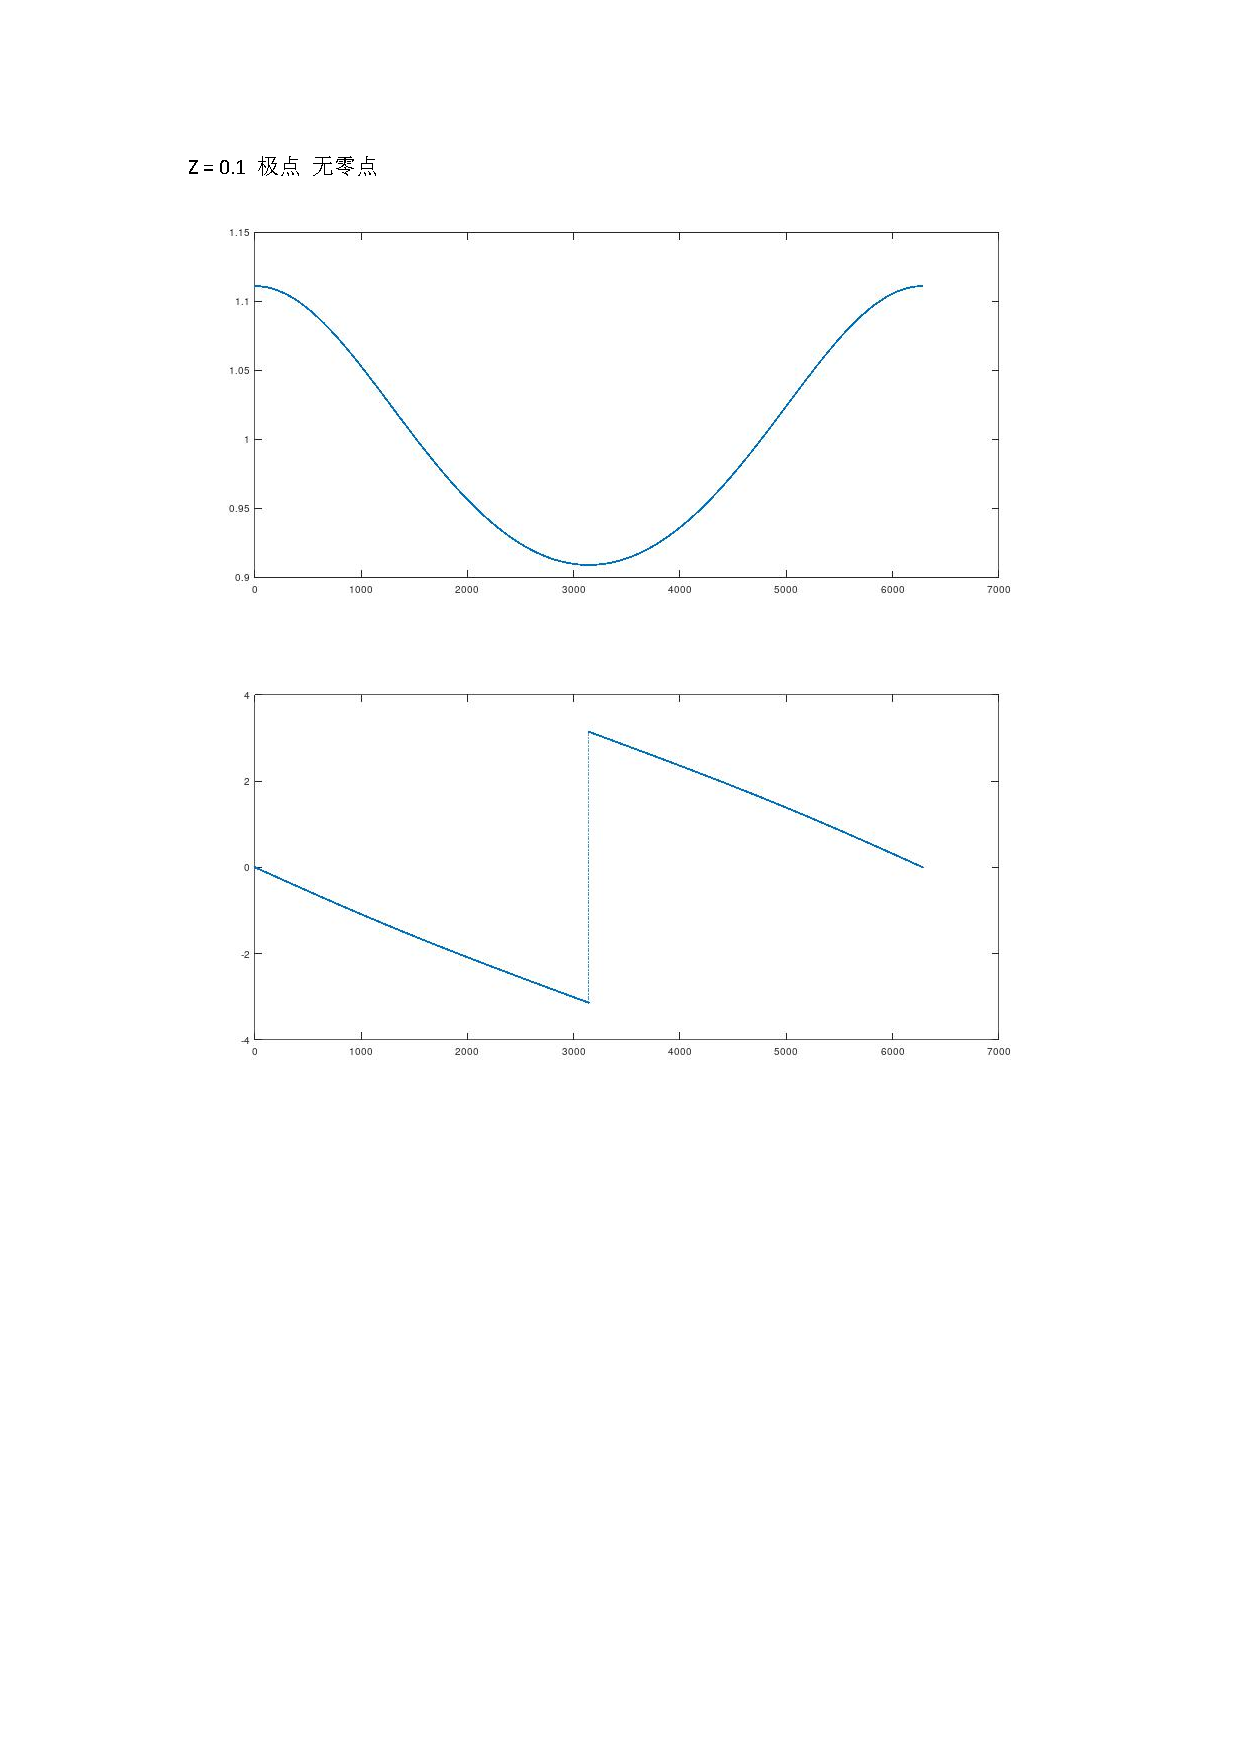
\includepdf[pages=-, pagecommand={}]{../figure/zp.pdf}
% End Here


\let\chapname\undefined
\ifx\mainclass\undefined
\end{document}
\fi 